\documentclass[a4paper,10pt]{article}
\usepackage[utf8]{inputenc}
\usepackage[margin=1in]{geometry}
\geometry{left=0.5in,right=0.5in,top=0.5in,bottom=0.5in}
\usepackage{enumitem}
\usepackage{hyperref}
\usepackage{fancyhdr}
\usepackage{titlesec}
\usepackage{tikz}
\usepackage{array}
\usetikzlibrary{shapes, arrows.meta}

% \pagestyle{fancy}
% \fancyhf{}
% \fancyhead[L]{\small Ningkun Zhou}
% \fancyhead[R]{\small \thepage}

\hypersetup{
    colorlinks=true,
    linkcolor=blue,
    filecolor=magenta,      
    urlcolor=blue,
}

\titleformat{\section}{\large\bfseries}{\thesection}{1em}{}
\titlespacing*{\section}{0pt}{2ex}{1ex}

% Define a command for the horizontal line with optimized thickness
\newcommand{\sectionline}{
  \vspace{-2ex}
  \noindent
  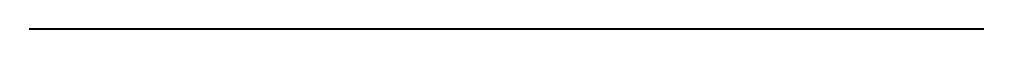
\begin{tikzpicture}
  \draw[thick] (0,0) -- (\textwidth,0);
  \end{tikzpicture}
}

% Adjust spacing between sections
\titlespacing{\section}{0pt}{2ex}{1ex}

\begin{document}
\begin{center}
    \textbf{\Huge Ningkun Zhou} \\
    \vspace{1mm}
    \begin{tabular}{@{}l@{\hspace{2em}}l@{\hspace{2em}}l@{\hspace{2em}}l@{}}
        \texttt{\href{mailto:nkzhou26@gmail.com}{nkzhou26@gmail.com}} & 
        \texttt{+(86) 150-1045-9923} & 
        \texttt{\href{https://www.linkedin.com/in/ningkun-zhou-087983177/}{LinkedIn}} & 
        \texttt{\href{https://github.com/nzhou26}{https://github.com/nzhou26}} \\  
    \end{tabular} \\
    \vspace{1mm}
    Machine Learning Engineer with \textbf{5 years of experience}, specializing in computer vision applications in industrial and scientific settings
\end{center}

% Education Section
\section*{EDUCATION}
\sectionline
\noindent
\begin{tabular*}{\textwidth}{@{}p{0.795\textwidth}@{}p{0.25\textwidth}@{}}
\textbf{B.Sc. Genetics and Computer Sciences} & \textbf{Sep 2015 -- May 2019} \\ 
\textit{University of Wisconsin, Madison} &
\end{tabular*}
    

% Work Experience Section
\section*{WORK EXPERIENCE}
\sectionline
\noindent
\begin{tabular*}{\textwidth}{@{}p{0.805\textwidth}@{}p{0.25\textwidth}@{}}
\textbf{Algorithm Engineer} - \textit{Danieli China} & \textbf{Apr 2022 -- Jul 2024} 
\end{tabular*}
Developed Deep Learning-based Automatic Scrap Classification system for multiple steel plants.
\begin{itemize}
    \item \textbf{Auto-adaptive PTZ camera}: I developed an auto-adaptive image acquisition system designed to consistently capture unique, high-resolution zoomed-in images. Leveraging \textbf{YOLO}, \textbf{Deep SORT tracking} and \textbf{image registration} algorithms, the system precisely identifies new layers of exposed scrap for detailed imaging. Each zoomed-in image maintains a stable scale, matching the width of the unloading truck. This stability is achieved through a \textbf{PTZ vs. XY-Mag} calibration algorithm that I developed.
    \item \textbf{Scrap Net}: Customized and fine-tuned popular \textbf{instance segmentation} architectures to production level, handling large quantities of annotation data, exceeding 25,000 images and \textbf{100,000 polygons} per dataset. Decoupled the original software into multiple API and MQ-based \textbf{microservices}, which enhanced system stability. Collaborated closely with customers to optimize the recognition system, achieving an accuracy rate of \textbf{90\% to 95\%}. Under my leadership of the algorithm team, our product have dominated the domestic market, with over 5 projects successfully accepted.
    \item \textbf{Innovations:}
    \begin{itemize}
        \item \textbf{CLIP}: Fine-tuned and deployed the CLIP model to reduce the need for extensive image classification annotations by encoding text prompts and image features. 
        Achieved a 30\% higher accuracy compared to the baseline EfficientNet model with the same amount of annotated data, reaching a 90\% accuracy with only 200 images.
        \item \textbf{Bale Breaker}: Developed the \textbf{first-in-market} quality assessment system for automatic monitoring of the scrap metal bale breaking process. Implemented \textbf{mechanical arms} to capture multi-angle interior images without disrupting on-site operations once the bale is dismantled. Achieved a classification accuracy of 95\%.
    \end{itemize}
\end{itemize}

\noindent
\begin{tabular*}{\textwidth}{@{}p{0.798\textwidth}@{}p{0.25\textwidth}@{}}
\textbf{Research Assistant} - \textit{Chinese Academy of Sciences, GIBH}  & \textbf{Jun 2019 -- Apr 2022}
\end{tabular*} 
Employed both conventional and innovative methods to resolve protein structures.
\begin{itemize}
    \item \textbf{Cryo-EM} [1],[2]: Applied advanced cryogenic-electron microscopy techniques to resolve multiple protein structures, 
                                managing all phases from data collection, particle extraction, \textbf{unsupervised clustering}, to reconstruction of 2D projections into 3D density maps and atomic-level protein model building. 
                                Contributed to two publications in high-impact journals, with \textbf{co-first author} status on one.
    \item \textbf{Cryo Check}: Developed a deep learning-based tool for cryo-EM micrograph quality assessment, facilitating \textbf{real-time} evaluation during Cryo-EM data collection. This innovative approach significantly reduced time and eliminated human bias in the selection of raw EM data. \href{https://github.com/nzhou26/cryoCheck}{https://github.com/nzhou26/cryoCheck}
    \item \textbf{Particle Seg}: Semantic segmentation tool for cryo-EM particles. It accurately segments a cryo-EM particle into three parts: signal, background, and edge. From the segmented ROI, for some cases, final resolution could be improved by 0.5 angstrom. \href{https://github.com/nzhou26/particleSeg}{https://github.com/nzhou26/particleSeg} 
\end{itemize}

% Skills Section
\section*{SKILLS}
\sectionline
\vspace{-4ex}
\begin{itemize}
    \item \textbf{Machine Leaning}: EfficientNet, U-Net, Mask R-CNN, YOLO, K-means clustering, CLIP
    \item \textbf{Programming}: Python (Tensorfow, Pytorch, Detectron2, Numpy, Pandas, Matplotlib), SQL, Bash
    \item \textbf{Miscellaneous}: Linux, Docker, Redis, RabbitMQ, RESTful API, PLC, Socket
    % \item \textbf{Specialization}:  Integrating of machine learning algorithms in PTZ camera
\end{itemize}

% Publications Section
\section*{PUBLICATIONS}
\sectionline
\vspace{-4ex}
\begin{enumerate}[leftmargin=0.15in]
    \item S. Dong, H. Li, \textbf{N. Zhou}, et al., ``Structural basis of nucleosome deacetylation and DNA linker tightening by Rpd3S histone deacetylase complex,'' \emph{Cell Research}, 2023. DOI: \href{https://doi.org/10.1038/s41422-023-00869-1}{10.1038/s41422-023-00869-1}.
    \item L. Tang, S. Dong, \textbf{N. Zhou}, et al., ``Vibrio parahaemolyticus prey targeting requires autoproteolysis-triggered dimerization of the type VI secretion system effector RhsP,'' \emph{Cell Reports}, 2022. DOI: \href{https://doi.org/10.1016/j.celrep.2022.111732}{10.1016/j.celrep.2022.111732}.
\end{enumerate}

\end{document}
